\section{Demo Implementation}
The implementation of the fluid solver demo created for this project is based primarily on Stam's later work on fluid dynamics for games~\cite{stam2003real}.
This paper gives a more practical implementation of the solver described by Stam.
This uses a concept known as smoke density, which can easily be visualised. 
This is a grid between zero and one, where zero indicates that no smoke is present and one indicates that it is consumed with smoke.
The demo uses this density function to visualise smoke in the scene. 

It was decided to focus on creating a 2D scene which used Stam's fluid equations to create smoke like effects.
The domain is limited to a square, as done by Stam~\cite{stam2003real}.
This square is of length $N+2$ as the extreme grid cells are used to either prevent smoke from leaving the box, or wrapping the smoke around in on itself and have to be treated specially.

\begin{figure}
  \caption{The 2D environment broken into an $(N+2) * (N+2)$ grid.}
  \centering
    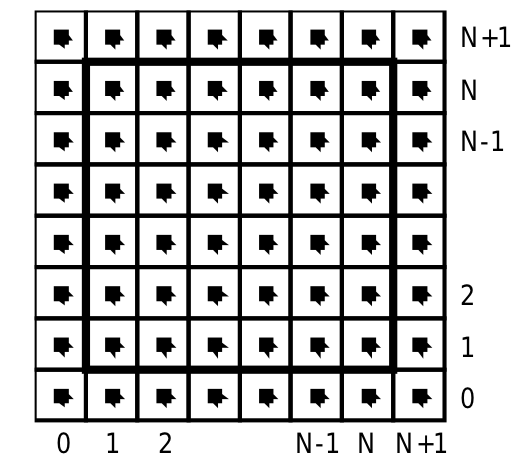
\includegraphics[width=0.5\textwidth]{images/grid}
\end{figure}

The velocity and the density at each grid cell is constant.
The velocity and densities are stored in 1D arrays for efficiency reasons.
The arrays are of length $size = (N+2) * (N+2)$ and array elements are accessed using the method in listing~\ref{ls1}.
\lstinputlisting[label=ls1,caption=Array index function, language=java]{code/ix.java}

The demo contains the environment within the 0.0 - 1.0 range on the x and y axes, so each grid cell has size $ h = 1 / N $.
The variable dt contains the fixed timestep between iterations.

\begin{figure*}
\centering
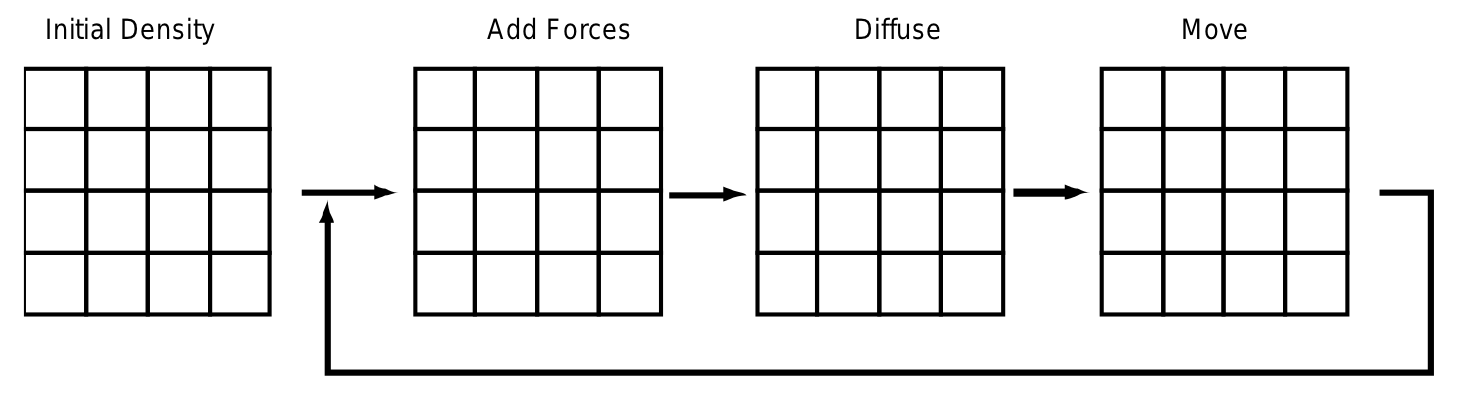
\includegraphics[width=1\textwidth]{images/density_solver}
  \caption{Structure of density solver, the three right hand terms are evaluated at each time step.}
\end{figure*}

The three right hand terms match up with the three terms on the right-hand side of the density Navier Stokes equation:
\begin{equation}
  \frac{\partial \rho}{\partial t} = -(u \cdot \nabla)\rho + \kappa \nabla^{2}\rho + S
\end{equation}

The theory for implementing the density solver is very similar to the velocity solver described previously.
The first term is simply the addition of sources of density based on the timestep, this allows users to add density dynamically.
\lstinputlisting[label=ls1,caption=Add Density source function, language=java]{code/source.java}

The second term represents the diffusion of density through the system which can be done by Gauss-Seidel relaxation.
This involves trying to extrapolate the densities which when we go back in time yield the current densities.
This has the same property as the method of characteristics in that it is stable.
\lstinputlisting[caption=Diffusion function, language=java]{code/diffuse.java}

The next stage of our density solver is the advection step which forces the density to follow a given velocity field.
We use a simple linear backtrace to determine the density which will follow the velocity field. 
This works by modelling the density as particles, and knowing that these particles will carry with them an amount of density which is retrieved by linear interpolating the density forwards in time based on the previous density values.
\lstinputlisting[caption=Advection step, language=java]{code/advect.java}

This is the density solver description in full.
Some of the functions have been modified for the demo for additional features as can be seen in the full source code.

We now turn our attention to the velocity solver, which reuses some of the functions from the density solver such as ``addSource'', ``diffuse'' and ``advect''.
It also adds in another function ``project'' which forces the velocity to be mass conserving. 
As described earlier, mass conserving fluids have the important property that they produce realistic swirly-like flows.
The routine uses a concept known as the Hodge decomposition~\cite{pirashvili2000hodge}.
This means that every velocity field is the sum of a mass conserving field and a gradient field.
To obtain an incompressible field we subtract the gradient field from our current velocities.
This involves computing the result of a Poisson equation which is done by Gauss-Seidel relaxation again.
The implementation is in the source code and will not be listed here for brevity.

When I had the initial implementation of the velocity and density solvers created as a demo in Processing, I decided to add some additional functionality.
For instance it is possible to add dynamic obstacles, toggle between visualising the velocity and density fields, and also visualising the density fields as a multicoloured gas to produce a flame-like effect.
